\section{Overview}
To ease the maintenance and ensure scalability, we have structured the project in an architecture which supports this.
The architecture consists of four macro components and a database, as can be seen in \cref{fig:architecture}. The macro components are: Shared, Location Service, Model Agent, and Web Service.\alexander{Maybe change the component name of `Model Updater' so it does not conflict with the layer name? \alexander{Changed name of component to `Model Agent'.}}

%\begin{figure}[h]
%\center
%\begin{tikzpicture}[
	path/.style={
		->,
		>=stealth
	},
	every node/.style={font=\sffamily,minimum height=1cm},
	database/.style={
	      cylinder,
	      cylinder uses custom fill,
	      shape border rotate=90,
	      aspect=0.25,
	      draw
	      }
]

% Webservice

\node[draw,circle,minimum size=1cm,inner sep=0pt, xshift=1cm,yshift=-3cm] (V){V};

\node[draw,circle,minimum size=1cm,inner sep=0pt,  xshift=-1cm,yshift=-3cm] (M){M};

\node[draw,circle,minimum size=1cm,inner sep=0pt, above=of V, xshift=-1cm] (C){C};

\node[above=of C, yshift=-1cm](webservice){Web Service};

\draw ($ (webservice.north west) + (-0.8,0.3) $) rectangle ($ (V.south east)+(0.6,-0.6) $);



\node[draw,minimum width=4cm,below=of V, yshift=-1.5cm,
xshift= -2cm,](model){Model};

\node[draw,minimum width=3cm,yshift=0.3cm,left=of model,rotate=90](updater){Model Updater};

% Data
\node [
draw,
below=of model,
minimum width=4cm,
] (data) {Data};

\node[database,below=of data
](database){Database};

\node[above=of updater.north east,yshift=-1cm,xshift=0.7cm](persistency){Business logic};

\draw ($ (persistency.north west) + (-0.3,0.3) $) rectangle ($ (data.east)+ (database.south) - (data.south) +(0.3,-.9) $);

% Data import
\node[draw,minimum width=3cm,right=of model,xshift=0.5cm](datacollector){Data Collector};

% Interface

\node[draw,below=of datacollector](locationsource){Location source};
\node[draw,right=of datacollector, rotate=90,anchor=south,xshift=-1cm,yshift=-0.5cm, minimum width=3cm](common){Common};

\node[above=of datacollector, yshift=-1.2cm,xshift=-0.9cm](dataloading){Data loading};



\draw ($ (dataloading.north west) + (-0.3,0.3) $) rectangle ($ (common.south west)+(0.3,-0.7) $);






% Connecting Arrows

\draw[path] (V.west) -- (M.east);
\draw[path] (C.south) -- (M.north);
\draw[path] (C.south) -- (V.north);

\draw[path] (datacollector.west) -- (model.east);
\draw[path] (datacollector.south) -- (locationsource.north);
\draw[path] (datacollector.east) -- (common.north);
\draw[path] (locationsource.east) -- (common.north);

\draw[path] (M.south) -- (model.north);
\draw[path] (model.south) -- (data.north);
\draw[path] (updater.south) + (0,1.2) -- (model.west);

\draw[path] (data.south) -- (database.north);

\end{tikzpicture}
%\caption{The architecture of the system}
%\label{arch}
%\end{figure}

\begin{figure}[H]
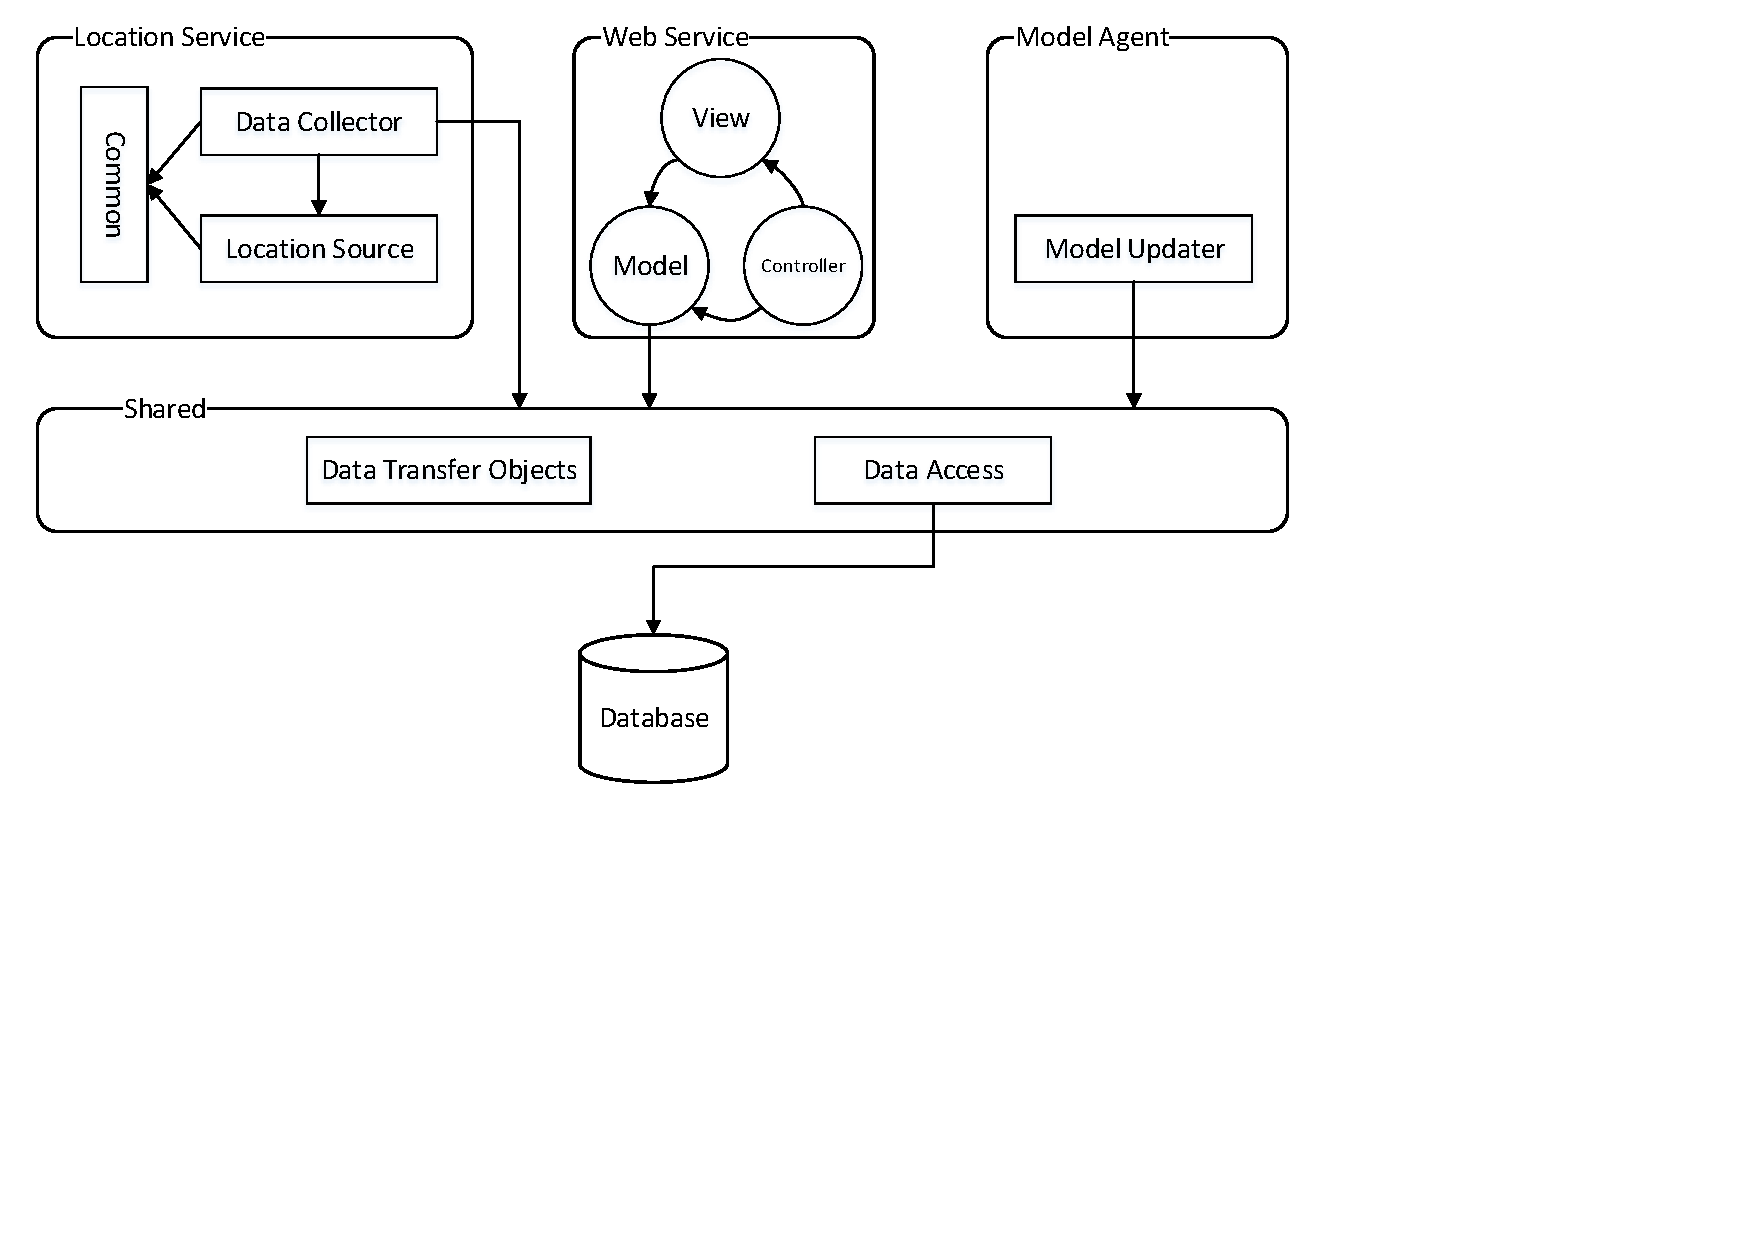
\includegraphics[width=\textwidth, trim={0 8.5cm 8cm 0}]{systemArchitecture.pdf}
\caption{The architecture of the system}
\label{fig:architecture}
\end{figure}

\subsection*{Database} The database used is a MySQL database, and is where all our data is stored.


\subsection*{Shared}\texttt{Shared} is the macro component containing the \texttt{Data Access} layer and the \texttt{Data Transfer Object} layer.

\paragraph{The Data Access layer} provides communication with the database.
All (SQL statements)/communication are encapsulated here providing the upper layers methods to communicate with the database.\alexander{Are `SQL statements' too implementation-specific?}\alexander{Reference to Database Design in appendix?}

\paragraph{The Data Transfer Object layer} contains all the shared data types and their attributes.
Using the \texttt{Data Transfer Object (DTO)} layer, data can be transfered between the \texttt{Web Service}, other macro components, and clients without several different data requests.\alexander{Is what we use really a DTO?}


\subsection*{Location Service}\texttt{Location Service} is the macro component containing the \texttt{Common} layer, the \texttt{Location Source} layer, and the \texttt{Data Collector} layer.
The macro component's task is to process and store location data directly from the data source. It is structured so the \texttt{Location Source} layer can easily be replaced.

\paragraph{The Common layer} encapsulates and describes the fetched data, making it easier for the \texttt{Location Source} layer and \texttt{Data Collector} layer to process.

\paragraph{The Location Source layer} fetched data from the data source then adapts and casts the data to the appropriate data type in the \texttt{Common} layer.

\paragraph{The Data Collector layer} gathers the data from the \texttt{Location Source} layer and processes it according to the standards of the \texttt{Data Transfer Object} layer. The data is then stored through the \texttt{Data Access} layer.


\subsection*{Model Agent}\texttt{Model Agent} is the macro component containing the \texttt{Model Updater} layer.

\paragraph{The Model Updater layer}


\subsection*{Web Service}\texttt{Web Service} is the macro component containing the \texttt{Model}, \texttt{View}, and \texttt{Controller}.

\paragraph{The Model} manages the data and actions possible for each data type.

\paragraph{The View} manages the display of data.

\paragraph{The Controller} handles the user input and sends commands to the \texttt{Model} and \texttt{View}.